% day-of-weeks.tex
% Author: Sébastien Combéfis
% Version: June 20, 2016

\documentclass[a4paper,11pt,final]{article}

% Packages
\usepackage[utf8x]{inputenc}
\usepackage[T1]{fontenc}
\usepackage[french]{babel}
\usepackage{lmodern}

\usepackage{graphicx}
\usepackage{tikz,pgf}
	\usetikzlibrary{arrows,decorations.pathreplacing}
\usepackage{array}
\usepackage{amssymb}
\usepackage{watermark}
\usepackage{xeCJK}
\usepackage{hyperref}
\usepackage{microtype}

% Page dimensions
\setlength\textheight{25.5cm}
\setlength\textwidth{17.5cm}
\setlength\oddsidemargin{-0.5cm}
\setlength\topmargin{-15mm}
\setlength\headheight{0mm}
\setlength\parindent{0.0cm}
\setlength\parskip{0.5cm}

% Style and fonts
\pagestyle{empty}
\urlstyle{sf}
\setmainfont{Cambria}
\setCJKmainfont{ipaexm.ttf}

% New colors
\definecolor{titleblue}{rgb}{0,0.2,0.4}
\definecolor{numberred}{rgb}{0.5,0,0}
\definecolor{sectionblue}{rgb}{0.1,0.3,0.7}
\definecolor{lightlightgray}{gray}{0.9}

% New commands
\renewcommand{\arraystretch}{1.3}
\newcommand{\trig}{\color{sectionblue}$\blacktriangleright$}
\newcommand{\sectit}[1]{\bigskip\hspace{-5mm}{\color{sectionblue}$\blacksquare$~~\Large\bfseries #1}}
\newcommand{\romaji}[1]{{\footnotesize[#1]}}

\begin{document}
	\rightwatermark{
		\begin{tikzpicture}[overlay]
			\draw[draw=none,fill=numberred] (17,-28.7) rectangle (18,-27.2);
			\node at (17.5,-27.8) {\color{white}\thepage};
			\node[anchor=west] at (-1.5,-28) {\raisebox{-0.5mm}{
\includegraphics[width=2cm]{images/by-nc-nd.pdf}}~~\small poly.glot, 2016.};
		\end{tikzpicture}
	}

% = = = = = = = = = = = = = = = = = = = = = = = = = = = = = = = = = = = = = = = = = = = = = = = = = = = =
% Jour de la semaine
% = = = = = = = = = = = = = = = = = = = = = = = = = = = = = = = = = = = = = = = = = = = = = = = = = = = =
\begin{tikzpicture}[overlay]
	\draw[draw=none,fill=titleblue] (4,-1) rectangle (19,1.5);
	\node[anchor=east] at (18,0.2) {\color{white}\Huge\sl Jour de la semaine};
	% https://openclipart.org/detail/183421/day-calendar
	\node[anchor=south east] at (2.5,-1.15) {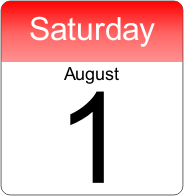
\includegraphics[width=2cm]{images/dayCalendar-200px.png}};
\end{tikzpicture}\vspace{15mm}
	
% - - - - - - - - - - - - - - - - - - - - - - - - - - - - - - - - - - - - - - - - - - - - - - - - - - - -

\og\textit{Jour}\fg{} se dit 日/ひ \romaji{hi} et on retrouve le kanji dans les jours de la semaine et \og\textit{semaine}\fg{} se dit しゅう \romaji{sh\=u}.

% - - - - - - - - - - - - - - - - - - - - - - - - - - - - - - - - - - - - - - - - - - - - - - - - - - - -

\sectit{De dimanche à samedi}

Les jours de la semaine se construisent à l'aide d'un élément (feu, bois, eau...) suivi de ようび \romaji{y\=obi} qui signifie tout simplement \og\textit{jour de la semaine}\fg. Cette façon de faire est spécifique aux japonais, et les mots suivants ne sont d'ailleurs \textbf{pas} utilisés en chinois.

\hspace{5mm}\begin{tabular}{|p{2cm}p{4.5cm}l}
	日曜日			& にちようび \romaji{nichiy\=obi}			& Dimanche \\
	月曜日			& げつようび \romaji{getsuy\=obi}			& Lundi \\
	火曜日			& かようび \romaji{kay\=obi}				& Mardi \\
	水曜日			& すいようび \romaji{suiy\=obi}			& Mercredi \\
	木曜日			& もくようび \romaji{mokuy\=obi}			& Jeudi \\
	金曜日			& きにょうび \romaji{kiny\=obi}			& Vendredi \\
	土曜日			& どようび \romaji{doy\=obi}				& Samedi
\end{tabular}

Au Japon, le premier jour de la semaine est le dimanche et il est associé au soleil. Les autres jours sont respectivement associés aux éléments suivants :

\begin{tabular}{*{7}{@{\qquad}c}}
	\Huge 日 & \Huge 月 & \Huge 火 & \Huge 水 & \Huge 木 & \Huge 金 & \Huge 土 \\
	soleil & lune & feu & eau & bois & métal & terre
\end{tabular}

% - - - - - - - - - - - - - - - - - - - - - - - - - - - - - - - - - - - - - - - - - - - - - - - - - - - -

\sectit{Vocabulaire}

\hspace{5mm}\begin{tabular}{|p{2cm}p{4.5cm}l}
	日				& ひ \romaji{hi}							& Jour \\
	週				& しゅう \romaji{sh\=u}					& Semaine \\
	曜日				& ようび \romaji{y\=obi}					& Jour de la semaine
\end{tabular}

On remarquera que 日 se prononce \romaji{hi} lorsqu'il est utilisé seul, mais \romaji{bi} dans 曜日.

\end{document}